
\begin{frame}
	\frametitle{Test Setup}
Several steps have been followed in order to enable the acquisition of meaningful data during the subjective tests. These steps include defining the test environment, choosing a rating framework and creating additional question that may help inferring informations about the participants and their way of rating content.


\large{Test Environment}
In order to make the results of our research reproducible we follow the ITU P.910 \cite{rec1998p} recommendation. 
The parameters include aspects such as viewing distance, peak luminance of the screen or background room illumination.
Performing tests following these specifications is common at the Technical University of Ilmenau, so we used a room meeting these requirements, which was already available.


	
\large{Rating Framework}
The testing procedure which seems most suited to this case is Absolute Category Rating (ACR) \cite{rec1998p}, where different versions of an original sequence are shown to a test participant. 

For each sequence the participant issues categorical ratings from any of these 5 answers: \{Excellent, Good, Fair, Poor, Bad\}

The steps performed by a participants during a rating session can be seen in the figure \ref{fig:workflow:state_machine}.

\begin{figure}[htb!]
	\centering
	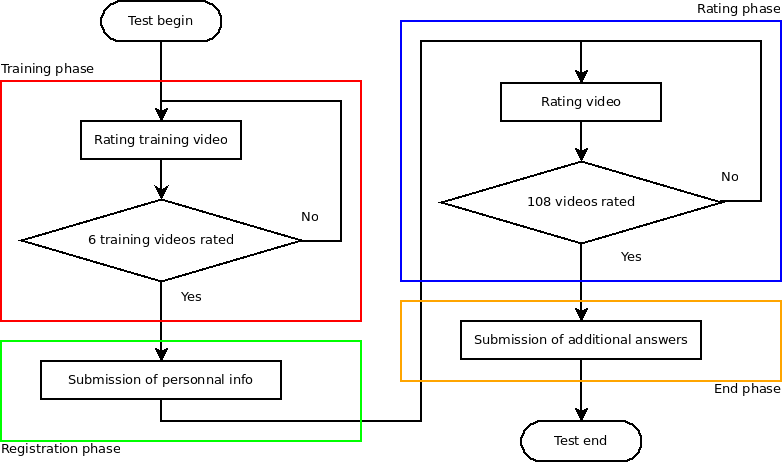
\includegraphics[width=3.5in]{rating_workflow}
	\caption{Detailed steps of a rating session}
	\label{fig:workflow:state_machine}
\end{figure}


\large{Additional collected data}
In order to gain more knowledge about the users behaviour, additional data is collected from the participants.

One of the suggestions of the ITU recommendation paper being the usage of several test questions in addition to the ratings \cite{rec1998p}, the following points have been assessed at the end of each rating session:
\begin{itemize}
	\item Impact of the following points on rating 
	\begin{itemize}
		\item Presence of blocky artifacts
		\item Visible bands of colour
		\item Smoothness of the playback
	\end{itemize}
	\item Exposure to 4k content and devices
	\item Confidence of the participant in his ratings
\end{itemize}

The idea behind these question is dual as they may translate how users perceive video features as well as how users may clearly express their perceptions. As it has been noticed in previous experiments and in discussions with test participants: users may still rate using a different scales, thus spreading the final \textit{MOS} or falsely being classified as outlier when their ratings may only represent a shift from the overall population. 

Moreover, mouse interactions have been collected during the rating of each sequence. The intent behind this is that as the MOS scale forbids detailed answers some participants may hesitate between two answers and change their final answer or hover over several ones before making his final choice.
Answering speed, which could be an indicator of a participant skipping answers or to the contrary being strongly confident in his answers is a feature that has been thought relevant to analyse. 
We believe that informations such as confidence in the participants ratings or more precise scores can be extracted from these previously described behaviours.


\large{Participants selection}
Extra care has been taken during participants selection in order to guarantee unbiased results. This selection process included dividing the participants selection between the different members of the research  group, recruiting participants from different student groups in the University and taking into account participants age and technical background.
\end{frame}